\documentclass[conference,10pt]{IEEEtran}

\usepackage{cite}
\usepackage{amsmath,amssymb}
\usepackage{graphicx}
\usepackage{tabularx}
\usepackage{placeins}
\usepackage{balance}
\usepackage{algorithm}
\usepackage{algpseudocode}
\usepackage[hidelinks]{hyperref}

% Keep figure descriptions in the source for future accessible output.
\newcommand{\Description}[1]{}
\setlength{\emergencystretch}{1em}


\title{Thermal-Aware NoC Reconfiguration for Concurrent General-Purpose Computing and MoE Inference in 3D-Stacked Systems}
\author{Anonymous Author(s)}

\begin{document}


\maketitle

\begin{abstract}
An asynchronous agent can run general-purpose tasks alongside AI inference. We focus on AI inference with mixture-of-experts (MoE) models. In a 3D DRAM-stacked system, MoE dispatch traffic can contend with general-purpose memory requests at shared network-on-chip (NoC) outputs, delaying a step that needs both results. We place coherence traffic on a separate Mesh and reconfigure MoE paths using predicted demand. Configurable switches provide additional MoE channels and bypass intermediate routers. Before updating routes, the controller estimates completion time, accounting for network interface delays, memory bank access, and reconfiguration overhead. Operator-level dynamic voltage and frequency scaling and thermal-aware task scheduling manage execution under peak-temperature constraints.
\end{abstract}

\begin{IEEEkeywords}
hybrid bonding, 3D integration, mixture-of-experts, network-on-chip,
reconfigurable interconnect, memory-bank contention, thermal management
\end{IEEEkeywords}
\raggedbottom

\section{Introduction}
\label{sec:introduction}

An asynchronous agent can run general-purpose tasks alongside AI inference.
A later step that needs both results must wait for both branches. In 3D
DRAM-stacked systems, high-bandwidth links connect the logic and memory
dies~\cite{li2026helios}, while the network-on-chip (NoC) carries token
exchanges between nodes hosting different experts in a mixture-of-experts
(MoE) model. General-purpose traffic and MoE dispatch bursts can contend for
the same router output. Frequent short memory requests can add substantial
load, and queueing can delay responses needed by the agent.

MoE token exchange can involve many nodes in a single batch. Uneven expert
activation can concentrate traffic on a few node pairs and saturate even
short paths, while distant transfers consume forwarding capacity across
multiple routers. The communicating nodes and heavily used paths change with
inputs, model layers, and the dispatch and combine phases. Thermal coupling
between the stacked logic and DRAM tiers can also trigger throttling and
prolong inference.

HiBand selects among four local/global bandwidth modes~\cite{wang2026hiband},
but mode selection alone does not choose dedicated connections for
individual heavy source--destination pairs. Flows with similar locality
can therefore remain on the same contended resources.

To address these problems, we propose a framework that combines
traffic-aware NoC reconfiguration with thermal-aware execution.
We separate coherence traffic onto a dedicated Mesh and add configurable
switches to the MoE Mesh. The switch connections change with communication
demand. A predictor estimates
per-phase demand, and a configuration algorithm assigns packets to compatible
circuits under switch-conflict and network interface and memory bank capacity
constraints. The controller checks estimated completion time and
reconfiguration overhead before applying an update. Operator-level
energy-aware DVFS and thermal-aware task scheduling support execution under
peak-temperature constraints.

This work makes three contributions:
\begin{enumerate}
  \item We design a reconfigurable NoC for concurrent general-purpose
  workloads and MoE inference in 3D DRAM-stacked systems. Separate Mesh
  planes carry coherence and MoE traffic. The switch fabric
  provides local channels and cross-region paths that can be reassigned to
  individual node pairs between communication phases.

  \item We develop a phase-dependent method that predicts demand, selects
  compatible circuits, and assigns packets within shared network interface
  and memory bank capacities. A completion-time check accounts for
  reconfiguration overhead.

  \item We evaluate how the design affects the modeled readiness of a step
  that waits for both the general-purpose and MoE branches. While keeping peak temperature below the specified threshold,
  the modeled time to readiness is reduced by up to 9.01\% relative to HiBand.
\end{enumerate}

\setlength{\textfloatsep}{12pt}
\setlength{\floatsep}{10pt}

\section{Motivation}
\label{sec:motivation}

\subsection{Target System and Workloads}
\label{sec:target-system-workloads}

\begin{figure}[!tbp]
  \centering
  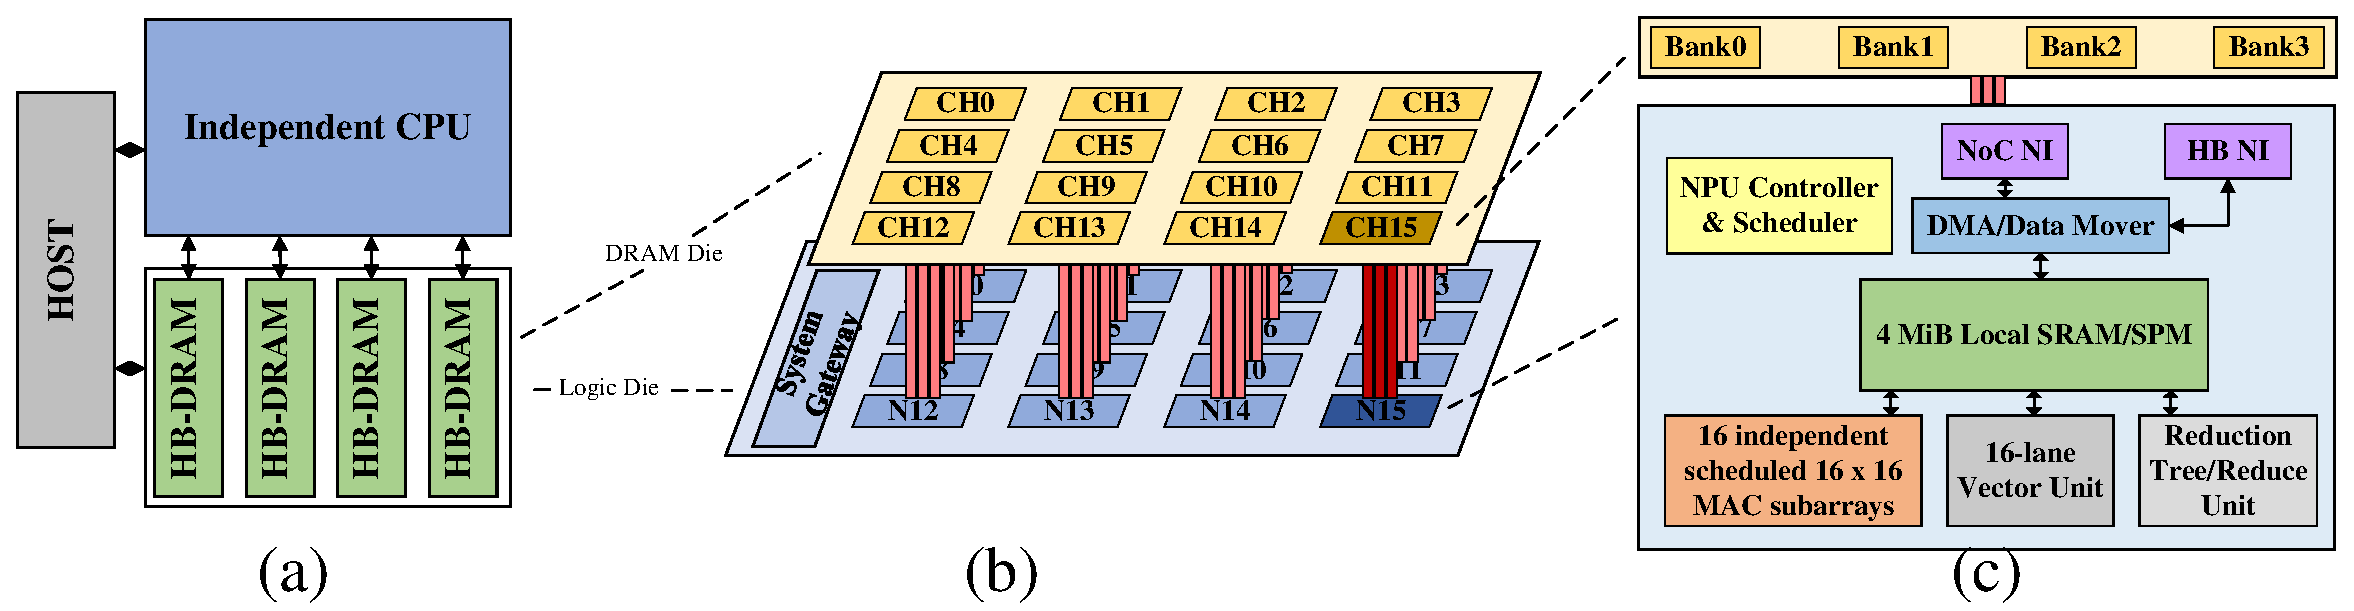
\includegraphics[width=\columnwidth]{figures/target_architecture_uniform_titles.pdf}
  \caption{Target 3D system. (a) Host and HB-DRAM organization. (b) Face-to-face
  integration of the $4\times4$ Logic-tier NPU mesh and the aligned DRAM
  channels. (c) Microarchitecture of an NPU--memory pair.}
  \Description{Three panels show the host and HB-DRAM organization, the
  vertically aligned NPU clusters and DRAM channels, and the internal
  organization of one NPU--memory pair.}
  \label{fig:target-architecture}
\end{figure}

Figure~\ref{fig:target-architecture} shows a 3D system in which the
logic and memory tiers are integrated by face-to-face hybrid bonding.
Each NPU cluster in the logic tier is vertically aligned with a DRAM
partition and accesses it through a local hybrid-bond link. A
horizontal $4\times4$ Mesh NoC connects the NPU clusters and carries
inter-cluster transfers, including MoE Dispatch and Combine traffic.
Local memory accesses and inter-cluster transfers therefore use distinct
physical paths. The stacked logic and DRAM dies are thermally coupled,
imposing a peak-temperature constraint on execution.

To study co-execution, we replay an MoE dispatch trace alongside synthetic
cache-coherence read requests that represent general-purpose memory traffic.
On the baseline, requests and responses share the horizontal Mesh with
MoE traffic.

The main MoE evaluation covers Qwen3-30B-A3B~\cite{qwen3report} and
Qwen1.5-MoE-A2.7B~\cite{qwen15moe} for language-model inference,
mini-SWE-agent~\cite{minisweagent} with a Qwen3-30B-A3B backend for
SWE-bench Lite tasks~\cite{swebench}, and LingBot TI2V~\cite{lingbotvideo}
for video generation.


\subsection{Cross-Workload Interference and MoE Hotspots}

\noindent\textbf{Problem.}
In the mesh, synthetic GetS (shared-read) requests and DataS
(data responses to shared-read requests) represent memory communication
from a concurrent general-purpose branch.
They enter through the modeled NIs and share router outputs with MoE
Dispatch/Combine packets. Figure~\ref{fig:noc-phenomenon}(a) compares
isolated execution, shared-Mesh co-execution, and dual-plane co-execution
with CSs disabled. Across 30 paired cases, the geometric-mean completion
ratios relative to each branch's isolated execution are 1.164/1.379 for
coherence/MoE on the shared Mesh and 1.135/1.365 on separate planes.
The geometric mean of the dual/shared ratios of summed stage-join
times is 0.977. Both configurations use the same traffic and NI/SRAM
service settings, with round-robin arbitration and CSs disabled.
Figure~\ref{fig:noc-phenomenon}(a) motivates separating coherence and MoE
traffic to reduce their mutual interference on shared Mesh resources.

\noindent\textbf{Root Cause.}
Packets requesting the same router output compete for finite link service.
Priority can redistribute waiting between branches. 
For parallel branches, stage readiness depends on the later completion,
$T_{\mathrm{join}}=\max(T_{\mathrm{coh}},T_{\mathrm{MoE}})$, measured
from a common time origin.
A response can therefore arrive earlier without advancing the stage if
MoE remains the last predecessor. Likewise, improving coherence service
by postponing MoE can increase the final join time. The relevant decision
must follow the dependency that releases the next step and account for
the completion of both branches.

Virtual channels, wider shared links, and temporal scheduling provide
other ways to manage concurrent traffic. Virtual channels can reduce
head-of-line blocking, while additional bandwidth can raise service
capacity and scheduling can change when traffic overlaps. Their benefit
depends on the resource budget and traffic pattern. The present
comparison motivates evaluating physical separation together with these
shared-resource constraints.

Within MoE communication, expert selection and placement concentrate
transfers on particular node pairs. Overlapping XY routes create hotspots
whose locations change across layers and communication phases.
Figure~\ref{fig:noc-phenomenon}(b) shows peak path-derived router demand
moving from R9 to R5 to R10 across layers 1, 24, and 48.
The heatmaps aggregate messages along their deterministic paths.
They identify spatial demand concentration, while measured queueing
and completion times establish its timing effect. Two phases with
similar total bytes can load different directed links because their
source--destination pairs differ. A configuration suitable for one
phase can consequently provide little benefit in the next.
Short routes can saturate at nearby destinations, while distant transfers
occupy several routers. Configurable paths should therefore accommodate
both local bandwidth demand and long-distance forwarding.


\begin{figure}[!t]
  \centering
  \begin{minipage}[t]{0.49\columnwidth}
    \vspace{0pt}\centering
    \parbox[c][7mm][c]{\linewidth}{\centering\fontsize{7}{8}\selectfont
    (a) Cross-workload\\Interference}\par
    \parbox[c][31mm][c]{\linewidth}{\centering
    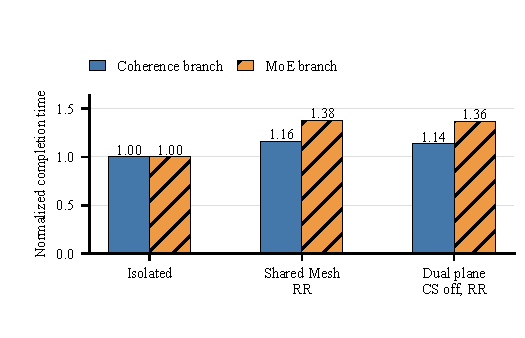
\includegraphics[width=\linewidth]{figures/fig2a_interference_compact.pdf}}
  \end{minipage}\hfill
  \begin{minipage}[t]{0.49\columnwidth}
    \vspace{0pt}\centering
    \parbox[c][7mm][c]{\linewidth}{\centering\fontsize{7}{8}\selectfont
    (b) Router demand\\across MoE layers}\par
    \parbox[c][31mm][c]{\linewidth}{\centering
    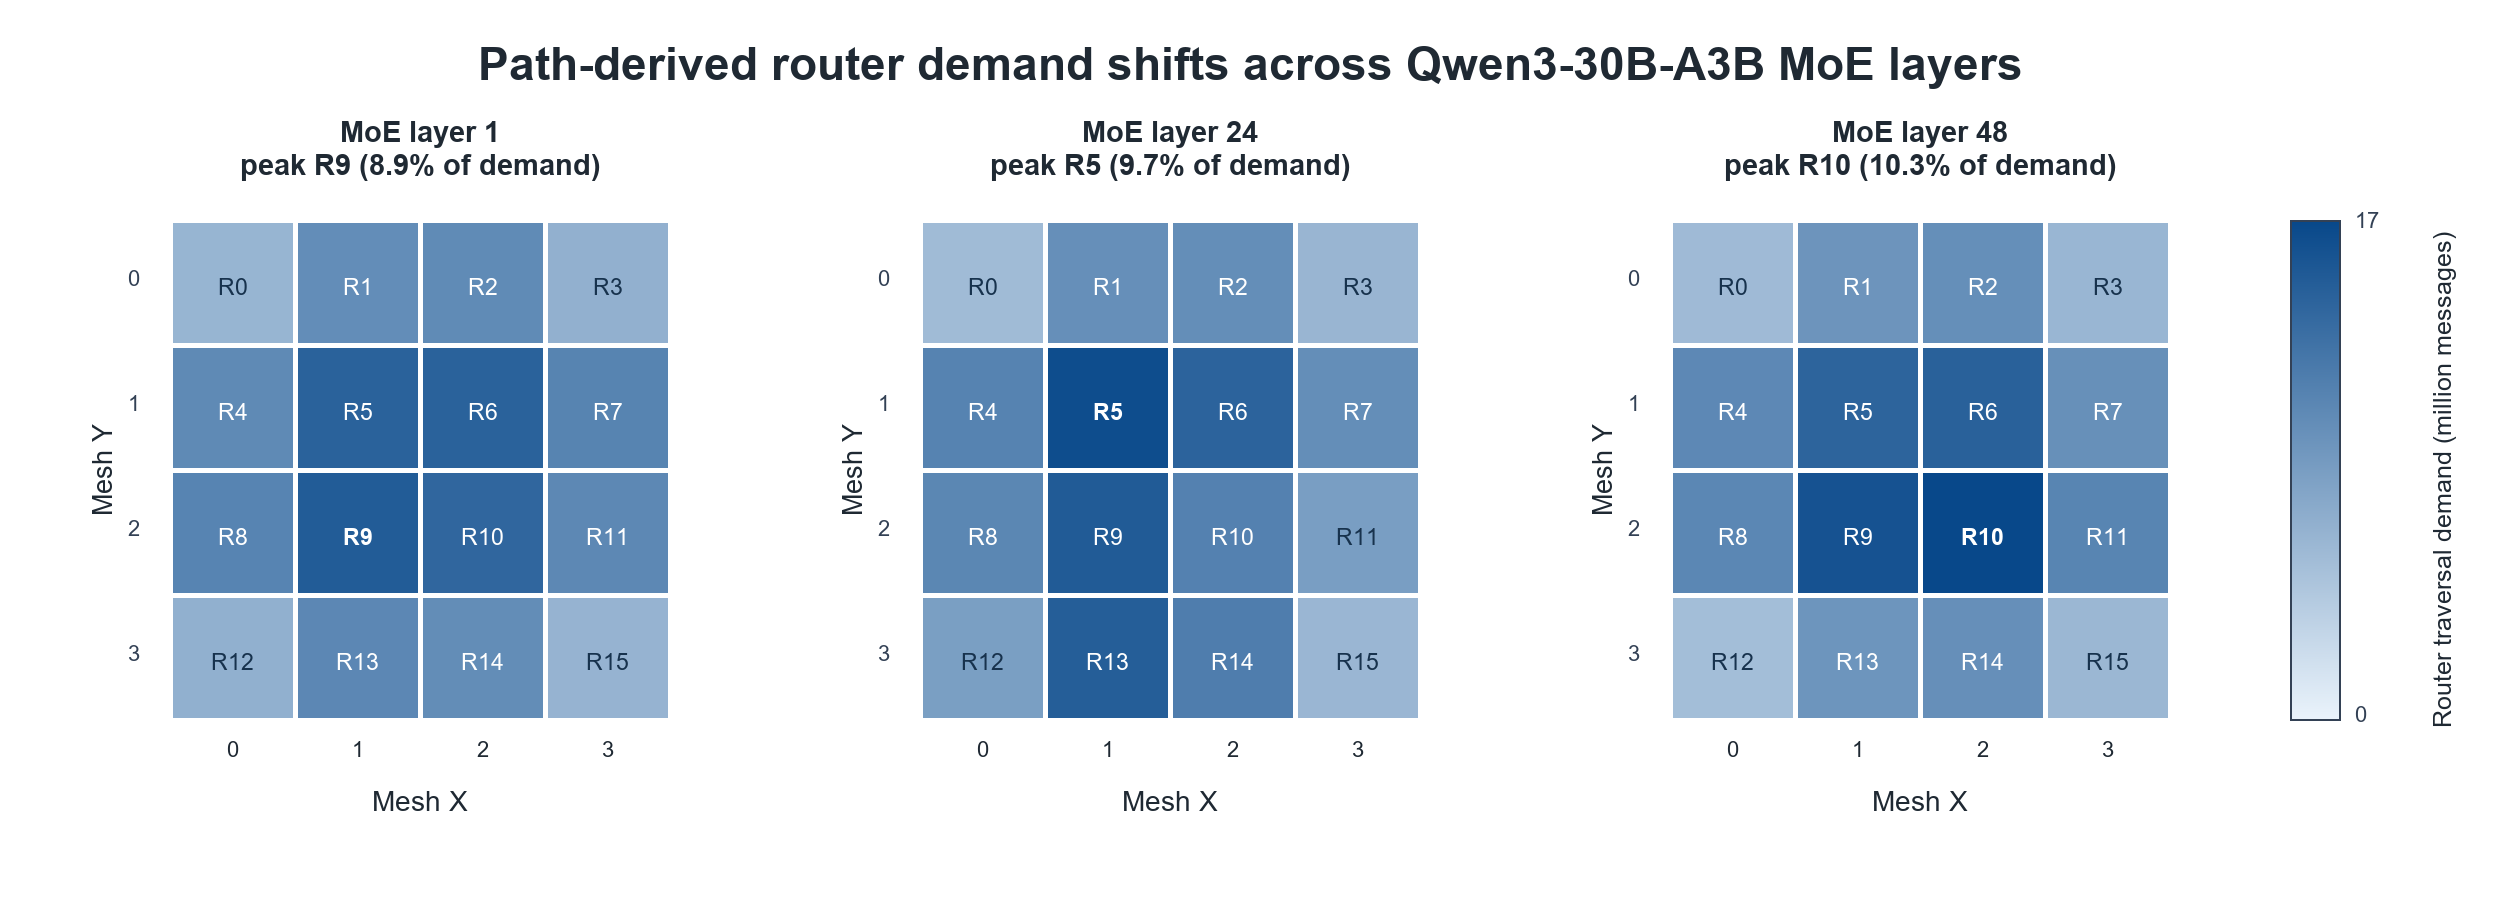
\includegraphics[width=\linewidth,trim=18bp 14bp 5bp 24bp,clip]{figures/noc_cause_router_hotspots_revised.png}}
  \end{minipage}
  \caption{(a) Branch completion times normalized to separate isolated
runs. Bars show geometric means across 30 paired cases, each summing
six independent communication phases. Dual-plane CSs are disabled.
The geometric-mean dual/shared join-time ratio is 0.977.
(b) XY-path router demand across MoE layers, using a shared color scale.}
\Description{Normalized coherence and MoE completion times and
layer-dependent router demand.}
\label{fig:noc-phenomenon}
\end{figure}

\noindent\textbf{Opportunity.}
Separate physical planes reduce cross-class contention at inter-router
links and outputs. 
NI and SRAM service remain shared, and the added network resources
must be included in hardware-cost comparisons.
Within the MoE plane, configurable circuits provide local channels and
bypass intermediate routers as busy node pairs change. An update is
useful when its completion-time benefit covers configuration and
remaining shared-resource costs.
A selected circuit can relieve a congested Mesh path while increasing
demand at its source NI, destination NI, or SRAM interface. Candidate
evaluation must propagate these waits through packet completion and
consumer readiness. The decision also includes the time required to
pause admissions, drain old transfers, install a configuration, and resume
injection. Retaining the active configuration remains appropriate when
the available communication window cannot recover these costs.

\noindent\textbf{Thermal Constraints.}
Contention and routing choices affect when computation and memory
operations proceed and may change the spatial and temporal distribution
of activity. Thermal coupling between logic and DRAM tiers makes peak
temperature a constraint on the resulting execution. We therefore combine
the NoC mechanisms with operator-level energy-aware DVFS and thermal-aware
task scheduling. These controls adjust frequency and task start times
under the temperature limit. Their thermal and execution-time effects are
evaluated through matched on/off comparisons.
A shorter communication phase can change the overlap of subsequent
operators, and activity on a different path can change where power is
dissipated. The resulting temperature trajectory depends on both the
power distribution and thermal history. We therefore evaluate temperature,
completion time, and energy together when assessing thermal control.

\section{Design}
\label{sec:design}

\subsection{Dual-Plane NoC}
\label{sec:noc-design}

Figure~\ref{fig:noc-physical-design} shows two physically separate
$4\times4$ networks on the logic tier. Plane M carries MoE data and
control messages through the original Mesh and configurable switches
(CSs). Plane C carries GetS shared-read requests and their DataS
responses. Each node $N_i$ connects directly to its corresponding
coherence router $C_i$. The interconnects are routed in the logic die's
metal layers.

The M plane retains nine lower CSs and four upper CSs. Each lower CS
connects to the four corner nodes of a $2\times2$ group. Corner, edge,
and interior nodes thus have one, two, and four CS attachments.
Upper switches $\mathrm{CS}_9$--$\mathrm{CS}_{12}$ form a $2\times2$
network and connect down to $\mathrm{CS}_0$, $\mathrm{CS}_2$,
$\mathrm{CS}_6$, and $\mathrm{CS}_8$, respectively. A local circuit
connects two NIs through one lower CS; a longer circuit uses the upper
network to bypass intermediate Mesh routers. MoE packets use an
assigned circuit or the M-plane Mesh. Coherence requests and responses
use C-plane links independently of these route choices.

\begin{figure}[!t]
  \centering
  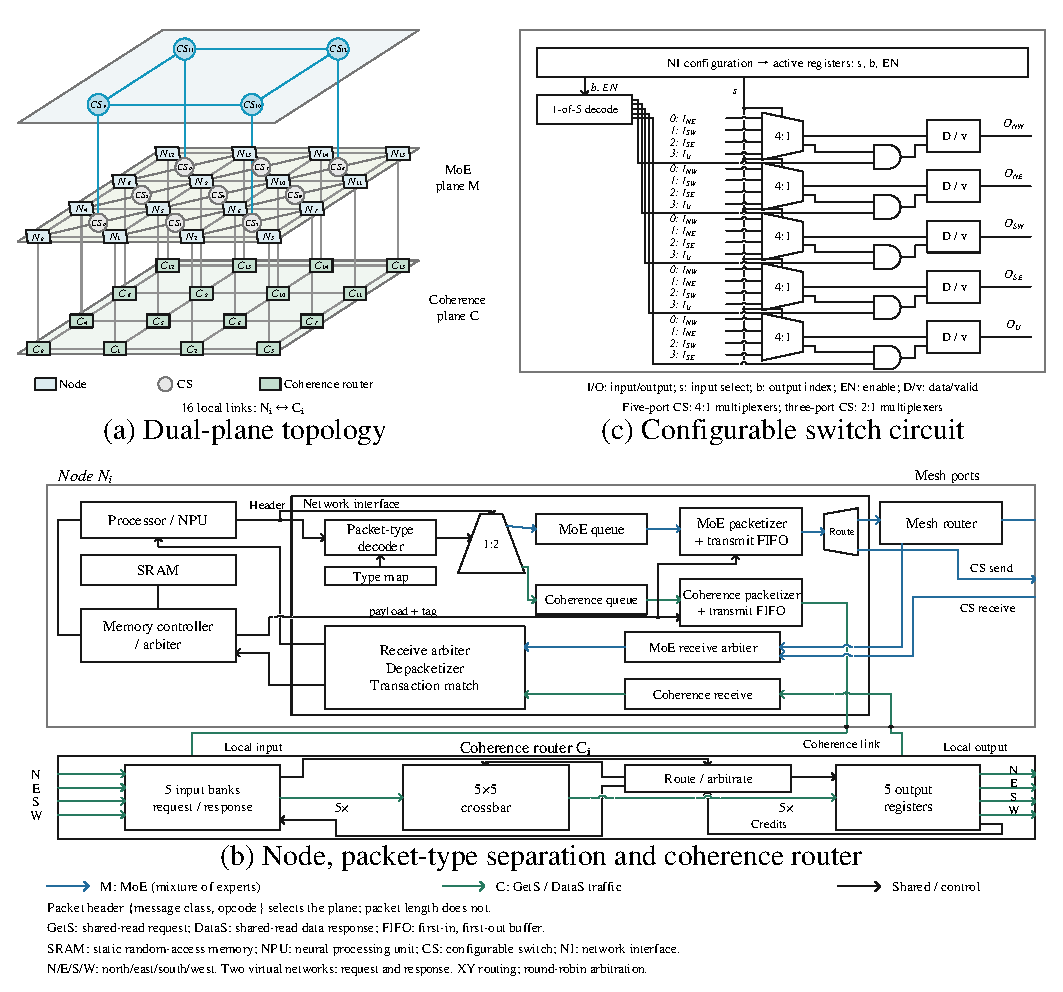
\includegraphics[width=\columnwidth]{figures/noc_dual_plane_uniform_titles.pdf}
  \caption{Dual-plane NoC. (a) MoE Mesh/CS plane M and coherence Mesh
  plane C, with one local connection per node.
  (b) Node, packet-type decoder, and five-port coherence router.
  (c) CS circuit with input selection and output enable.}
  \Description{The upper-left panel shows the two networks and sixteen
  node-to-coherence-router connections. The upper-right panel shows a
  five-direction configurable switch. The lower panel shows packet-type
  classification, separate MoE and coherence queues, packet formation,
  receive processing, shared SRAM arbitration, and the coherence router.}
  \label{fig:noc-physical-design}
\end{figure}

\subsection{Node and Network Interface}
\label{sec:noc-node-design}

Figure~\ref{fig:noc-physical-design}(b) shows an NPU node with banked
SRAM, a network interface (NI), and an M-plane Mesh router. The NI
decodes the message class and opcode before packet formation. Its type
map directs GetS and DataS to plane C and MoE messages to plane M.
A short MoE control message uses M, while a DataS response carrying a
cache line uses C. Separate queues and packetizers feed the two planes;
each packet keeps its selected plane throughout transmission.
Source reads, receive writes, and NPU accesses share the SRAM arbiter.

Each $C_i$ has four neighbor ports and one local NI port, with separate
input queues for requests and responses. These queues form two virtual
networks with independent credits. A $5\times5$ crossbar connects the
input banks to output registers. XY routing selects the next direction,
and round-robin arbitration selects an eligible input. Output registers
hold data until the receiver accepts it. The NI allocates response
storage before issuing GetS; the service endpoint reserves a response
transmit slot before starting the memory operation. Request and response
queues therefore have separate storage and flow-control state.

On plane M, the NI selects the Mesh or a configured CS attachment for
each complete packet. Packets carry a transfer identifier, byte offset,
and transfer length. Receive descriptors supply the destination SRAM
address. The receive arbiter and depacketizer check the packet and
write its payload at that address plus the offset. A receipt bitmap
records accepted writes, and completion is reported when all expected
packet writes finish. Finite receive queues buffer concurrent Mesh
and CS arrivals. The C-plane receive path matches responses to their
request identifiers and shares the endpoint's SRAM write service.

\subsection{Configurable Switches}
\label{sec:noc-switches}

Figure~\ref{fig:noc-physical-design}(c) shows a lower CS with directions
NW, NE, SW, SE, and U. Five four-input multiplexers select among the
other directions' inputs. The configuration fields $s$, $b$, and EN
select the input, output, and connection enable. Output decoding
activates one directed input--output pair. Data and valid propagate
forward, and ready propagates back along the selected connection.
The output register retains its data under backpressure.

Only $\mathrm{CS}_0$, $\mathrm{CS}_2$, $\mathrm{CS}_6$, and
$\mathrm{CS}_8$ have U links. The remaining lower CSs have their U
interfaces disabled. Each upper CS has two neighbor directions and
one downward direction, implemented with three two-input multiplexers.
Separate NI attachments permit concurrent MoE circuits, subject to
shared NI service, direct memory access (DMA) engines, and SRAM bandwidth.

\subsection{Traffic Prediction}
\label{sec:traffic-prediction}

GetS requests and DataS responses use XY routing on plane C. The host
optimizes MoE routes on plane M. For Dispatch, we adapt MixNet's
adjacent-layer predictor~\cite{liao2025mixnet}:
\begin{equation}
  \widehat{\mathbf y}_{\ell,s}=P_\ell\mathbf x_{\ell-1,s},
  \quad P_\ell\geq0,\quad
  \mathbf1^{\mathsf T}P_\ell=\mathbf1^{\mathsf T}.
  \label{eq:noc-load-prediction}
\end{equation}
Here $\mathbf x_{\ell-1,s}$ is the preceding layer's normalized expert distribution
for tokens with known source NI $s$. Weighted least squares fits $P_\ell$
from paired token groups, weighting their size and recency. Prefill and
decode use separate models, with a historical-mean fallback.
Expert placement and packing map forecasts to source--destination
demand. Final allocation uses actual Top-K and packing metadata.
Combine uses confirmed assignments, output shapes, and estimated
expert completion times to derive return packets and release times.

\subsection{Reconfiguration Problem}
\label{sec:noc-problem}

Within a fixed $H$-cycle planning interval, $\mathcal M_f$ contains
the unbound packets of MoE source--destination flow $f$.
Their payloads $b_m$ give $D_f=\sum_{m\in\mathcal M_f}b_m$ and
$\mathcal M=\bigcup_f\mathcal M_f$. Legal CS paths for packet $m$
form $\mathcal P_m$, with $\mathcal P=\bigcup_m\mathcal P_m$.
Each simple path connects the source and destination NI through wired
CS ports. Binary $z_p$ selects path $p$;
binary $x_{m,p}$ assigns packet $m$ to it. We maximize useful payload
assigned to the CS network:
\begin{equation}
  \max_{\mathbf z,\mathbf x}\quad
  V=\sum_{m\in\mathcal M}b_m\sum_{p\in\mathcal P_m}x_{m,p}.
  \label{eq:noc-volume-objective}
\end{equation}
Readiness flag $g_m$ equals one when source data and receive storage
are ready, and zero otherwise. Each packet uses at most one enabled path:
\begin{equation}
  \sum_{p\in\mathcal P_m}x_{m,p}\leq1,
  \qquad x_{m,p}\leq z_p,\quad x_{m,p}\leq g_m.
  \label{eq:noc-packet-assignment}
\end{equation}
Selected paths are CS-disjoint. With $A_{c,p}=1$ when $p$ uses CS $c$,
\begin{equation}
  \sum_{p\in\mathcal P}A_{c,p}z_p\leq1,
  \qquad c=0,\ldots,12.
  \label{eq:noc-cs-exclusion}
\end{equation}

Resource $r\in\mathcal R$ is an M-plane link or NI, DMA, or SRAM service.
Its remaining budget $C_r$ within $H$ deducts work outside $\mathcal M$:
existing transfers, configuration messages, and C-plane use of shared endpoints.
Cost $u_{m,p,r}$ includes framing and expresses service in NoC cycles.
Unassigned packets use the M-plane Mesh, denoted
by 0, with $x_{m,0}=1-\sum_{p\in\mathcal P_m}x_{m,p}$. Thus,
\begin{equation}
  \sum_{m\in\mathcal M}\sum_{p\in\mathcal P_m\cup\{0\}}
  u_{m,p,r}x_{m,p}\leq C_r,\qquad r\in\mathcal R.
  \label{eq:noc-resource-capacity}
\end{equation}
At most two paths are selected, $\sum_{p\in\mathcal P}z_p\leq2$;
a path may traverse multiple CSs.
Path $p$ specifies the input, output, and enable fields of each CS;
$x_{m,p}$ determines the source NI's route tag for packet $m$.

\subsection{Configuration Algorithm}
\label{sec:noc-algorithm}

Offline enumeration supplies local and upper-CS paths. We target the two
M-plane links with the largest pending MoE flit counts. For each link
still unrelieved, flows are visited in decreasing $D_f$, with endpoint
identifiers breaking ties. Up to $K_p=2$ paths per flow are tried by length
and then identifier. We retain the first CS-disjoint extension that passes
joint \textsc{Assign} and increases $V$. Construction ends after two paths,
both links, or budget exhaustion. At most two configurations are retained;
the one-path configuration remains available when a second path is added.

Candidates are checked in decreasing $V$. A timing model propagates
source reads, finite queues, credits, receive writes, and dependencies;
DataS follows its request's memory service. While $S_0$ forwards, an update
must satisfy, using the same time origin,
\begin{equation}
  \widehat T(S)+\eta(S)<\widehat T(S_0).
  \label{eq:noc-switching-check}
\end{equation}
Here $\eta(S)\geq0$ is calibrated from paired errors on held-out requests.
Protected consumers satisfy
$\widehat T_k(S)-\widehat T_k(S_0)+\eta_k(S)\leq\epsilon_k$,
including MoE with $\epsilon_k=0$ and coherence transactions with their
specified allowances. Estimates include controller execution, pause,
drain, writes, and NI installation. After pause acknowledgement and drain, versions and eligibility are refreshed and feasibility, timing, and budgets are
rechecked before Section~\ref{sec:noc-config-interface}'s update protocol.

\begin{algorithm}[H]
  \caption{CS configuration for at most two hotspots}
  \label{alg:noc-configuration}
  \small
  \begin{algorithmic}[1]
    \Require MoE packets $\mathcal M$, paths $\mathcal P$, budgets $C_r$, active $S_0$
    \Ensure $S_0$, an acknowledged update, or an update error
    \State $\mathcal H\gets$ up to two M-plane links with largest demand
    \State $S\gets$ Mesh allocation; $\mathcal C\gets\varnothing$
    \For{$e\in\mathcal H$ while construction budget remains}
      \State \textbf{if} $S$ already relieves $e$ \textbf{then continue}
      \State $S'\gets$ first feasible extension for $e$ increasing $V$, or $S$
      \If{$V(S')>V(S)$}
        \State $S\gets S'$; $\mathcal C\gets\mathcal C\cup\{S\}$
      \EndIf
      \State \textbf{if} two paths are selected \textbf{then break}
    \EndFor
    \For{$S'\in\mathcal C$ in decreasing $V$}
      \State \textbf{if} budget expired \textbf{then return} $S_0$
      \State Estimate completion and update overhead
      \If{timing checks pass within the decision budget}
        \State Request packet holds and pause new CS admissions
        \If{pause and drain complete within budget}
          \State Refresh state; recheck feasibility and timing
          \State \textbf{if} final checks pass \textbf{then return} $\Call{ApplyCS}{S'}$
        \EndIf
        \State Release holds and resume $S_0$; \Return $S_0$
      \EndIf
    \EndFor
    \State \Return $S_0$
  \end{algorithmic}
\end{algorithm}


\subsection{Configuration Interface}
\label{sec:noc-config-interface}

The host sends CS configuration commands over the M-plane Mesh.
Each lower CS is configured by its northwest node's NI; that CS relays
commands to its attached upper CS where present. A separate NI
configuration queue feeds the CS command decoder, which writes the
configuration register and returns an acknowledgement. This control
interface is independent of the selected CS data connection.

Table~\ref{tab:noc-command-fields} summarizes the command fields.
A lower CS uses three output-selection bits, two input-selection bits,
and one enable bit; an upper CS uses two, one, and one, respectively.
The output code follows the instance's wired directions, and the input
code indexes that output's allowed inputs. The NI stores each MoE
packet's assigned CS attachment and configuration version in its
transfer descriptor. Unassigned MoE packets use the M-plane Mesh.

\begin{table}[!t]
  \caption{CS configuration command fields.}
  \label{tab:noc-command-fields}
  \centering\small
  \begin{tabularx}{\columnwidth}{@{}p{0.25\columnwidth}>{\raggedright\arraybackslash}X@{}}
    \hline
    Field & Meaning \\
    \hline
    Type & Message class and operation code. \\
    Destination & NI responsible for the target CS. \\
    TransactionID & Command--response matching identifier. \\
    ConfigVersion & CS configuration and matching packet assignments. \\
    Target & CS index or NI transfer descriptor. \\
    Operation & Write, install descriptor, pause, status, or resume. \\
    State & CS input/output selection and enable, or packet assignments. \\
    Status & Success or failure of the requested operation. \\
    \hline
  \end{tabularx}
\end{table}

The NI acknowledges a pause after holding the selected unbound MoE
descriptors and stopping new CS admissions. Admitted transfers retain
their routes. After the final check, \textsc{ApplyCS} drains these
transfers, writes and confirms the CS states, installs matching NI
assignments and versions, and resumes transmission. A rejected final check
releases the holds and resumes $S_0$. A write or installation error
is reported with CS admissions paused until matching CS and NI
configurations are restored. Plane C continues forwarding throughout.

\subsection{Thermal-Aware Execution}
\label{sec:thermal-design}

Thermal-aware execution complements bank placement and
NoC reconfiguration by adjusting operator frequencies and
task start times to reduce latency under thermal constraints.
Let $s_j$ and $r_j$ denote the start time and frequency
ratio of task $j$. The execution objective is
\begin{equation}
\begin{aligned}
  \min_{\{s_j,r_j\}} \quad & T_{\mathrm{inf}} \\
  \mathrm{s.t.}\quad
  & T_b[k]\leq T_{\mathrm{limit}},\quad \forall b,k,
\end{aligned}
\label{eq:thermal-optimization}
\end{equation}
where $T_{\mathrm{inf}}$ is the inference completion time
and $T_b[k]$ is the temperature of physical block $b$ at
thermal sampling step $k$.
We address this objective through offline operator-level
energy-aware DVFS and runtime thermal-aware task scheduling.


\noindent\textbf{Operator-Level Energy-Aware DVFS.}
We profile each operator type at three DVFS settings, $r\in\{1.0,0.75,0.5\}$, with separate profiles for different execution configurations. For each profile, we select the frequency that minimizes total execution energy, including dynamic and idle energy. For operators with overlapping computation and memory accesses, reducing the frequency can lower energy consumption with little increase in execution time. This can reduce heat generation and mitigate thermal throttling during inference.

\noindent\textbf{Model-Based Thermal Scheduling.}
We use a HotSpot-based RC thermal model~\cite{hotspot_tool} to capture delayed heat propagation between the Logic and DRAM tiers. Rather than repeatedly performing full RC simulations during scheduling, we precompute the temperature responses of individual tasks, including delayed temperature peaks after task completion. At runtime, the controller evaluates the predicted temperatures of candidate tasks and selects the task with the earliest feasible start time.

\FloatBarrier

\section{Evaluation Results and Analysis}
\label{sec:experiment}

\subsection{Experimental Setup}
We model 16 hybrid-bonded NPU clusters, each with 4096 MACs, a 16-lane
vector unit, and 4~MiB SRAM, alongside 32~GiB HB-DRAM. The $4\times4$
Mesh uses 256-bit links at 1~GHz; each vertical link provides 25.6~GB/s.
The workloads are Qwen3-30B-A3B and Qwen1.5-MoE-A2.7B (prefill/decode),
mini-SWE-agent with Qwen3 (model calls and Agent tasks), and LingBot TI2V
(video generation). Paired runs match input, precision, arrivals, and
initial state. For concurrent tasks, stage join waits for both compute
and coherence responses.

\subsection{Performance Comparison}
Figure~\ref{fig:eval-overall} shows stage-join reductions of
5.74\%, 9.01\%, 7.15\%, and 8.17\% relative to HiBand~\cite{wang2026hiband}
for Qwen3, mini-SWE-agent, LingBot TI2V, and Qwen1.5, respectively.
Latency reduction is $1-T_{\mathrm{design}}/T_{\mathrm{HiBand}}$.
The comparison covers modeled communication stages. Layer measurements and
end-to-end estimates have different completion boundaries.

\begin{figure}[!t]
\centering
\begin{minipage}[t]{0.49\columnwidth}
\centering\vspace{0pt}
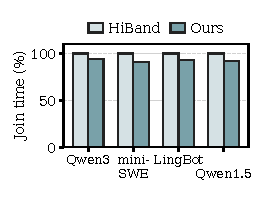
\includegraphics[width=\linewidth]{figures/fig5_performance_halfcolumn.pdf}
\caption{Stage-join time relative to HiBand (100\%).}
\Description{Grouped bars compare normalized stage-join time for four workloads.}
\label{fig:eval-overall}
\end{minipage}\hfill
\begin{minipage}[t]{0.49\columnwidth}
\centering\vspace{0pt}
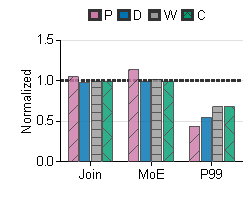
\includegraphics[width=\linewidth]{figures/fig6a_ablation.pdf}
\caption{Communication ablation relative to shared-Mesh RR.}
\Description{Twelve bars compare three normalized metrics for P, D, W, and C.}
\label{fig:eval-breakdown}
\end{minipage}
\end{figure}

\subsection{Ablation and Implementation Overhead}
Figure~\ref{fig:eval-breakdown} separates traffic-plane, arbitration, and circuit
effects using the common RTL/endpoint testbench. Five frozen Qwen1.5-MoE
transport inputs comprise one each at 4 and 8 tokens and three 16-token seeds.
Hotspot/distributed GetS placement and aggregate release intervals of 1, 3,
and 6 cycles give 30 development conditions. Bank waiting is fixed at eight
cycles; payloads, arrival plans, queues, and shared NI/SRAM service budgets
are matched. Each communication phase starts from a fresh network, so their
completion-time sum is not end-to-end inference latency. Ratios are computed
per condition before geometric averaging; these conditions reuse five inputs
and are not independent replicate samples.

\paragraph{Traffic separation and arbitration}
Under RR, the dual plane with CS disabled reduces the join-time sum by
2.32\% relative to shared Mesh, with 20 conditions improving and ten tying.
This benefit includes the additional C-plane resources; it is not an
equal-area comparison. On shared Mesh, fixed type priority reduces the
worst-phase GetS P99 by 56.43\%, but increases the MoE and join-time sums by
13.06\% and 4.44\%, respectively. Earlier responses therefore need not
advance joint completion. Priority uses a separately built, reviewed RTL
revision; the driver, inputs, and service budgets are unchanged. It is an
alternative arbitration control, not a step in the CS configuration chain.

\paragraph{Circuit paths and configuration waiting}
Forced CS increases join time by 0.79\% relative to the CS-off dual plane.
To isolate its path effect, a control applies the same configuration commands
and holds the same selected packets, but keeps their payloads on Mesh.
Configuration counts and start/end times match in all 180 phases. This
matched-wait control increases join time by 1.31\% over CS-off, while forced
CS shortens time by 0.52\% relative to that control. Thus, a small path benefit
can be offset by configuration and selected-packet waiting. Injection-order
interactions make these effects non-additive. Recorded configuration
intervals are 845--925 simulated cycles, distinct from the separate
architecture model's 40-cycle aggregate installation parameter.

\paragraph{Online-policy boundary}
The charged-host-time runtime prototype commits no updates in the 180
main-matrix phases: each phase completes during candidate construction.
Its completion times equal those of CS-off and are not plotted again.
Forced-CS results characterize the routing mechanism rather than established
online-policy gains. The ablation does not establish dual-plane type-priority
performance or real adjacent-layer prediction accuracy.

\paragraph{Sensitivity}
Stage-join changes by token count, GetS placement, and release interval:
xxx. Configuration-cost and decision-lead sweeps (ranges and results):
xxx.

\noindent\textbf{Thermal ablation.}
In the modeled 24-layer Qwen1.5-MoE run (four requests, 512 prefill and
one decode token each), both arms use fixed XY Mesh, a common warm state
(63.501~$^{\circ}$C peak), and no bank-conflict optimization. Enabling DVFS
and thermal scheduling reduces peak temperature from 64.985 to
63.968~$^{\circ}$C; both satisfy the 65~$^{\circ}$C cap for this batch.
Completion time increases from 6.658 to 7.771~s (+16.72\%) and energy
from 49.491 to 51.544~J (+4.15\%).

Table~\ref{tab:eval-cost} compares simplified shared-Mesh and C/M network
cores, excluding full endpoints, SRAM/banks, distributed configuration,
thermal, and cross-tier hardware. FPGA: Vivado 2017.4, XCKU5P, 200~MHz
OOC post-route timing. ASIC: Yosys 0.23, Nangate45 TT, 1~ns constraint,
synthesis area. We report configuration delay for the 16-token hotspot and
distributed cases, in that order (seed 641103, one GetS per cycle). The
metric is $100(T_{\mathrm{cfg}}-T_{\mathrm{pre}})/T_{\mathrm{cfg}}$, using the
six-phase join sums with timed configuration ($T_{\mathrm{cfg}}$) and with
preinstallation ($T_{\mathrm{pre}}$). The control preserves the CS image,
packet assignments, and input releases and omits timed configuration
traffic and selected-packet holds.

\begin{table}[!ht]
\caption{Network-core and runtime costs (simplified NIs).}
\label{tab:eval-cost}
\centering\scriptsize
\renewcommand{\arraystretch}{0.85}
\begin{tabularx}{\columnwidth}{@{}>{\raggedright\arraybackslash}Xrr@{}}
\hline
Metric & Shared Mesh & Dual plane + CS \\
\hline
FPGA LUTs / flip-flops & 31,995 / 38,286 & 117,625 / 92,783 \\
FPGA BRAM / DSP & 0 / 0 & 0 / 0 \\
FPGA setup WNS (ns), 200\,MHz & $+0.339$ & $+0.043$ \\
ASIC synthesis area (mm$^2$) & 0.332176 & 0.869972 \\
ASIC area increase (\%) & --- & 161.90 \\
\hline
Exposed decision overhead (\%) & xxx & xxx \\
Exposed configuration delay (\%) & --- & 0.51 / 0.49 \\
\hline
\end{tabularx}
\end{table}

\FloatBarrier

\section{Related Works}
\label{sec:related-works}

\paragraph{Reconfigurable NoCs and traffic management}
SMART~\cite{krishna2013smart} enables packets to bypass multiple routers
within a cycle, reducing traversal latency. HiBand~\cite{wang2026hiband}
reallocates local and global bandwidth through four NoC modes for
HB-DRAM inference. Application-aware prioritization~\cite{das2009priority}
ranks packets according to their applications' stall-time criticality.
These studies address traversal cost, bandwidth allocation, and
shared-resource arbitration. Our design combines separate coherence and
MoE planes with configurable MoE circuits, selecting connections according
to communication demand and checking their effect on consumer completion time.

\paragraph{MoE communication and memory optimization}
ExpertFlow~\cite{he2026expertflow} combines routing prediction, token
scheduling, and expert caching to reduce parameter transfers during
memory-constrained inference. MixNet~\cite{liao2025mixnet} adapts an
optical-electrical fabric to changing expert communication demands in
distributed MoE training. HBSpec~\cite{wang2026hbspec} uses
communication-aware mapping and operator scheduling for hybrid-bonded
speculative decoding. Together, these studies demonstrate the importance
of coordinating computation and data movement. Our work applies demand
prediction to on-chip circuit allocation and accounts for network interface
capacity, memory bank access, and reconfiguration overhead when evaluating
concurrent general-purpose tasks and MoE inference.

\paragraph{Thermal management in 3D systems}
Tasa~\cite{he2025tasa} addresses thermal constraints in 3D-stacked LLM
systems through cross-stack thermal optimization and bandwidth sharing.
Thermal-aware scheduling has also been studied for controlling runtime
temperature in 3D multicore processors~\cite{tsai2016thermal}.
Our thermal mechanism combines operator-level energy-aware DVFS with
scheduling based on predicted temperature responses. It accounts for
delayed heat propagation between logic and DRAM tiers. The thermal
ablation uses common NoC and endpoint-service settings in both runs.

\par\addvspace{5pt}
\section{Conclusion}
\label{sec:conclusion}

We presented thermal-aware NoC reconfiguration for concurrent
general-purpose computing and MoE inference in 3D-stacked systems.
Separate traffic planes and configurable MoE circuits adapt communication
paths to changing demand. A completion-time check accounts for memory
access and reconfiguration costs, while operator-level DVFS and
thermal-aware scheduling manage execution under temperature constraints.
The evaluation quantifies communication-stage gains and the trade-off
between peak temperature, latency, and energy under thermal control.

\clearpage
\balance
\bibliographystyle{IEEEtran}
\bibliography{references,thermal_references}

\end{document}

